%%
%% This is file `sample-manuscript.tex',
%% generated with the docstrip utility.
%%
%% The original source files were:
%%
%% samples.dtx  (with options: `manuscript')
%% 
%% IMPORTANT NOTICE:
%% 
%% For the copyright see the source file.
%% 
%% Any modified versions of this file must be renamed
%% with new filenames distinct from sample-manuscript.tex.
%% 
%% For distribution of the original source see the terms
%% for copying and modification in the file samples.dtx.
%% 
%% This generated file may be distributed as long as the
%% original source files, as listed above, are part of the
%% same distribution. (The sources need not necessarily be
%% in the same archive or directory.)
%%
%% Commands for TeXCount
%TC:macro \cite [option:text,text]
%TC:macro \citep [option:text,text]
%TC:macro \citet [option:text,text]
%TC:envir table 0 1
%TC:envir table* 0 1
%TC:envir tabular [ignore] word
%TC:envir displaymath 0 word
%TC:envir math 0 word
%TC:envir comment 0 0
%%
%%
%% The first command in your LaTeX source must be the \documentclass command.
%%%% Small single column format, used for CIE, CSUR, DTRAP, JACM, JDIQ, JEA, JERIC, JETC, PACMCGIT, TAAS, TACCESS, TACO, TALG, TALLIP (formerly TALIP), TCPS, TDSCI, TEAC, TECS, TELO, THRI, TIIS, TIOT, TISSEC, TIST, TKDD, TMIS, TOCE, TOCHI, TOCL, TOCS, TOCT, TODAES, TODS, TOIS, TOIT, TOMACS, TOMM (formerly TOMCCAP), TOMPECS, TOMS, TOPC, TOPLAS, TOPS, TOS, TOSEM, TOSN, TQC, TRETS, TSAS, TSC, TSLP, TWEB.
% \documentclass[acmsmall]{acmart}

%%%% Large single column format, used for IMWUT, JOCCH, PACMPL, POMACS, TAP, PACMHCI
% \documentclass[acmlarge,screen]{acmart}

%%%% Large double column format, used for TOG
% \documentclass[acmtog, authorversion]{acmart}

%%%% Generic manuscript mode, required for submission
%%%% and peer review
\documentclass[manuscript,screen,review]{acmart}
%% Fonts used in the template cannot be substituted; margin 
%% adjustments are not allowed.
%%
%% \BibTeX command to typeset BibTeX logo in the docs
\AtBeginDocument{%
  \providecommand\BibTeX{{%
    \normalfont B\kern-0.5em{\scshape i\kern-0.25em b}\kern-0.8em\TeX}}}

%% Rights management information.  This information is sent to you
%% when you complete the rights form.  These commands have SAMPLE
%% values in them; it is your responsibility as an author to replace
%% the commands and values with those provided to you when you
%% complete the rights form.
\setcopyright{acmcopyright}
\copyrightyear{2018}
\acmYear{2018}
\acmDOI{XXXXXXX.XXXXXXX}

%% These commands are for a PROCEEDINGS abstract or paper.
\acmConference[Conference acronym 'XX]{Make sure to enter the correct
  conference title from your rights confirmation emai}{June 03--05,
  2018}{Woodstock, NY}
%
%  Uncomment \acmBooktitle if th title of the proceedings is different
%  from ``Proceedings of ...''!
%
\acmBooktitle{Woodstock '18: ACM Symposium on Neural Gaze Detection,
 June 03--05, 2018, Woodstock, NY} 
\acmPrice{15.00}
\acmISBN{978-1-4503-XXXX-X/18/06}


%%
%% Submission ID.
%% Use this when submitting an article to a sponsored event. You'll
%% receive a unique submission ID from the organizers
%% of the event, and this ID should be used as the parameter to this command.
%%\acmSubmissionID{123-A56-BU3}

%%
%% For managing citations, it is recommended to use bibliography
%% files in BibTeX format.
%%
%% You can then either use BibTeX with the ACM-Reference-Format style,
%% or BibLaTeX with the acmnumeric or acmauthoryear sytles, that include
%% support for advanced citation of software artefact from the
%% biblatex-software package, also separately available on CTAN.
%%
%% Look at the sample-*-biblatex.tex files for templates showcasing
%% the biblatex styles.
%%

%%
%% The majority of ACM publications use numbered citations and
%% references.  The command \citestyle{authoryear} switches to the
%% "author year" style.
%%
%% If you are preparing content for an event
%% sponsored by ACM SIGGRAPH, you must use the "author year" style of
%% citations and references.
%% Uncommenting
%% the next command will enable that style.
%%\citestyle{acmauthoryear}

%%
%% end of the preamble, start of the body of the document source.
\begin{document}

\title{Task 6  Numerical Methods}
\author{Carl-Emil Rohde \\ kvb125@alumni.ku.dk}
\date{September 2023}

\maketitle

\section{Problem 1}
\subsection{6.1.1}

\textbf{b.} Given the points $\left(x_0, y_0\right)=(7,146),\left(x_1, y_1\right)=(1,2)$, and $\left(x_2, y_2\right)=(2,1)$ :
\\
First, I find the divided differences $f\left[x_0, x_1\right], f\left[x_1, x_2\right]$, and $f\left[x_0, x_1, x_2\right]$.
\\
$$
\begin{aligned}
& f\left[x_0, x_1\right]=\frac{y_1-y_0}{x_1-x_0}=\frac{2-146}{1-7}=\frac{-144}{-6}=24 \\
& f\left[x_1, x_2\right]=\frac{y_2-y_1}{x_2-x_1}=\frac{1-2}{2-1}=\frac{-1}{1}=-1 \\
& f\left[x_0, x_1, x_2\right]=\frac{f\left[x_1, x_2\right]-f\left[x_0, x_1\right]}{x_2-x_0}=\frac{-1-24}{2-7}=\frac{-25}{-5}=5
\end{aligned}
$$
Now, the polynomial in Newton form is:
$$
\begin{aligned}
& P(x)=y_0+f\left[x_0, x_1\right]\left(x-x_0\right)+f\left[x_0, x_1, x_2\right]\left(x-x_0\right)\left(x-x_1\right) \\
& P(x)=146+24(x-7)+5(x-7)(x-1) \\
& P(x)=146+24 x-168+5 x^2-40 x+35 \\
& P(x)=5 x^2-16 x+13
\end{aligned}
$$
So the polynomial of least degree that interpolates the given data points is $P(x)=5 x^2-$ $16 x+13$
\\
\textbf{c.} First i arrange the data in increasing order of $x$:
$$
\begin{array}{l||r|r|r|r}
x & 1 & 2 & 3 & 7 \\
\hline y & 2 & 1 & 10 & 146
\end{array}
$$
Then I Calculate the first, second, and third order forward differences of y:
\\
\textbf{First-order differences:}
- $\Delta y_0=1-2=-1$
- $\Delta y_1=10-1=9$
- $\Delta y_2=146-10=136$
\\
\textbf{Second-order differences:}
- $\Delta^2 y_0=9-(-1)=10$
- $\Delta^2 y_1=136-9=127$
\\
\textbf{Third-order differences:}
- $\Delta^3 y_0=127-10=117$
\\
Then i use these to form the Newton interpolating polynomial $P(x)$:
$$
\begin{aligned}
P(x) & =y_0 \\
& +\left(x-x_0\right) \frac{\Delta y_0}{1 !} \\
& +\left(x-x_0\right)\left(x-x_1\right) \frac{\Delta^2 y_0}{2 !} \\
& +\left(x-x_0\right)\left(x-x_1\right)\left(x-x_2\right) \frac{\Delta^3 y_0}{3 !}
\end{aligned}
$$
Then i substitute the calculated and given values:
$$
\begin{aligned}
P(x) & =2 \\
& +(x-1)(-1) \\
& +(x-1)(x-2) \frac{10}{2} \\
& +(x-1)(x-2)(x-3) \frac{117}{6} \\
& =2-(x-1)+5(x-1)(x-2)+19.5(x-1)(x-2)(x-3)
\end{aligned}
$$
This is the interpolating polynomial of least degree for the given data set, in Newton's form.
\subsection{6.1.16}
\textbf{My pesudocode:}
\\
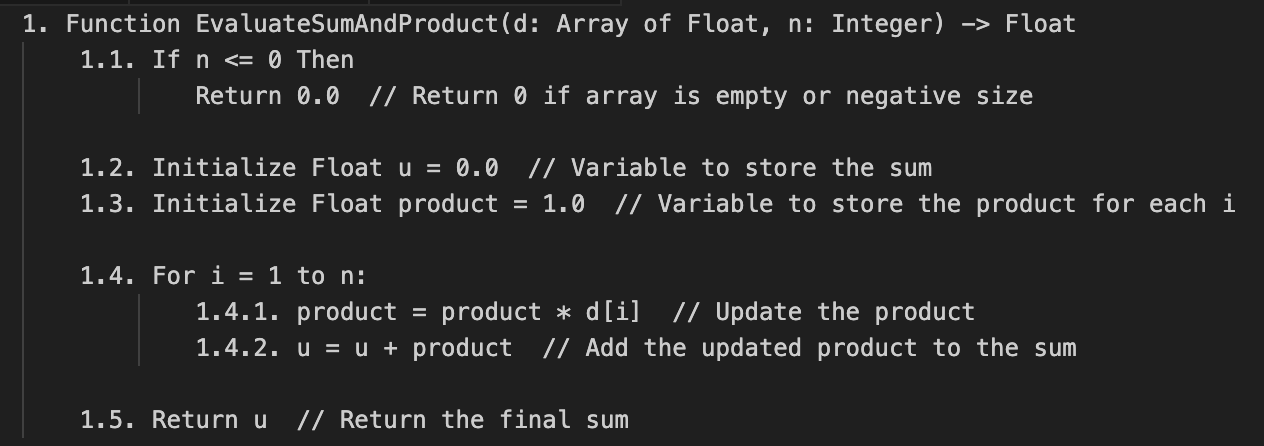
\includegraphics[width=0.65\linewidth]{12.png}
\\
\textbf{Explanation:}
\\
We initialize ' $u$ ' to 0 and 'product' to 1. We then loop through $i$ from 1 to $n$.
Inside the loop, we multiply the existing 'product' by $d[i]$ to get the product for the current
i. We add this to ' $u$ '. This avoids the need for a nested loop, and we get each term in the sum by doing just one multiplication and one addition. Therefore, the time complexity is $O(n)$, which is more efficient than the naive $O\left(n^2\right)$ approach.

\subsection{7.1.6}
I'll find the Taylor series expansions for each term in the approximation formula:
\\
1. $f(x+2 h)$
$$
f(x+2 h)=f(x)+2 h f^{\prime}(x)+\frac{(2 h)^2}{2 !} f^{\prime \prime}(x)+\frac{(2 h)^3}{3 !} f^{\prime \prime \prime}(x)+\frac{(2 h)^4}{4 !} f^{(4)}(x)+\mathcal{O}(h^5)
$$
2. $f(x+h)$
$$
f(x+h)=f(x)+h f^{\prime}(x)+\frac{h^2}{2 !} f^{\prime \prime}(x)+\frac{h^3}{3 !} f^{\prime \prime \prime}(x)+\frac{h^4}{4 !} f^{(4)}(x)+\mathcal{O}\left(h^5\right)
$$
3. $f(x-h)$
$$
f(x-h)=f(x)-h f^{\prime}(x)+\frac{h^2}{2 !} f^{\prime \prime}(x)-\frac{h^3}{3 !} f^{\prime \prime \prime}(x)+\frac{h^4}{4 !} f^{(4)}(x)+\mathcal{O}\left(h^5\right)
$$
4. $f(x-2 h)$
$$
f(x-2 h)=f(x)-2 h f^{\prime}(x)+\frac{(2 h)^2}{2 !} f^{\prime \prime}(x)-\frac{(2 h)^3}{3 !} f^{\prime \prime \prime}(x)+\frac{(2 h)^4}{4 !} f^{(4)}(x)+\mathcal{O}(h^5)
$$
\\
I then substitute these expansions into the original formula:
\\
$\begin{aligned} f^{\prime}(x) \approx & \frac{1}{12 h}[-f(x+2 h)+8 f(x+h)-8 f(x-h)+f(x-2 h)] \\ = & \frac{1}{12 h}\left[-\left(f(x)+2 h f^{\prime}(x)+\frac{4 h^2}{2 !} f^{\prime \prime}(x)+\frac{8 h^3}{3 !} f^{\prime \prime \prime}(x)+\frac{16 h^4}{4 !} f^{(4)}(x)\right)\right. \\ & +8\left(f(x)+h f^{\prime}(x)+\frac{h^2}{2 !} f^{\prime \prime}(x)+\frac{h^3}{3 !} f^{\prime \prime \prime}(x)+\frac{h^4}{4 !} f^{(4)}(x)\right) \\ & -8\left(f(x)-h f^{\prime}(x)+\frac{h^2}{2 !} f^{\prime \prime}(x)-\frac{h^3}{3 !} f^{\prime \prime \prime}(x)+\frac{h^4}{4 !} f^{(4)}(x)\right) \\ & \left.+\left(f(x)-2 h f^{\prime}(x)+\frac{4 h^2}{2 !} f^{\prime \prime}(x)-\frac{8 h^3}{3 !} f^{\prime \prime \prime}(x)+\frac{16 h^4}{4 !} f^{(4)}(x)\right)\right]\end{aligned}$
\\
After substituting, we need to simplify the terms:
\\
$\begin{aligned} f^{\prime}(x) \approx & \frac{1}{12 h}\left[-f(x)-2 h f^{\prime}(x)-2 h^2 f^{\prime \prime}(x)-\frac{4 h^3}{3} f^{\prime \prime \prime}(x)-\frac{4 h^4}{3} f^{(4)}(x)\right. \\ & +8 f(x)+8 h f^{\prime}(x)+4 h^2 f^{\prime \prime}(x)+\frac{8 h^3}{3} f^{\prime \prime \prime}(x)+\frac{2 h^4}{3} f^{(4)}(x) \\ & -8 f(x)+8 h f^{\prime}(x)-4 h^2 f^{\prime \prime}(x)+\frac{8 h^3}{3} f^{\prime \prime \prime}(x)-\frac{2 h^4}{3} f^{(4)}(x) \\ & \left.+f(x)-2 h f^{\prime}(x)+2 h^2 f^{\prime \prime}(x)-\frac{4 h^3}{3} f^{\prime \prime \prime}(x)+\frac{4 h^4}{3} f^{(4)}(x)\right] \\ = & \frac{1}{12 h}\left[12 h f^{\prime}(x)+\mathcal{O}\left(h^5\right)\right] \\ = & f^{\prime}(x)+\mathcal{O}\left(h^4\right)\end{aligned}$
\\
The error term for the approximation $f^{\prime}(x)$ is $\mathcal{O}\left(h^4\right)$, which shows that the approximation is fourth-order accurate.
\subsection{7.3.4}
To verify that this equation is a correct Gaussian formula, I can check if it gives exact results for polynomials of degree up to $2 n+1$, which in this case is 3 . Essentially, we are checking if the equation holds for $f(x)=1, f(x)=x, f(x)=x^2$, and $f(x)=x^3$:
\\
1. $f(x)=1$
$$
\begin{gathered}
\int_{-1}^1 1 d x=2 \quad \\
f(-\alpha)+f(\alpha)=1+1=2 \quad
\end{gathered}
$$
2. $f(x)=x$
$$
\begin{gathered}
\int_{-1}^1 x d x=0 \quad  \\
f(-\alpha)+f(\alpha)=-\frac{1}{\sqrt{3}}+\frac{1}{\sqrt{3}}=0 \quad}
\end{gathered}
$$
3. $f(x)=x^2$
$$
\begin{gathered}
\int_{-1}^1 x^2 d x=\frac{2}{3} \quad \\
f(-\alpha)+f(\alpha)=\left(-\frac{1}{\sqrt{3}}\right)^2+\left(\frac{1}{\sqrt{3}}\right)^2=\frac{2}{3}
\end{gathered}
$$ 
4. $f(x)=x^3$
$$
\begin{array}{r}
\int_{-1}^1 x^3 d x=0 \quad \\
f(-\alpha)+f(\alpha)=\left(-\frac{1}{\sqrt{3}}\right)^3+\left(\frac{1}{\sqrt{3}}\right)^3=0
\end{array}
$$
Since the formula holds for these polynomials, we can conclude that Equation (8) is a correct Gaussian formula for $n=1$.
\subsection{problem 2}
plotted the function $f(t)=e^{-t} \sin \left(\frac{\pi t}{2}\right)$ on the interval $[0,5]$ using $30 x$-values:
\\
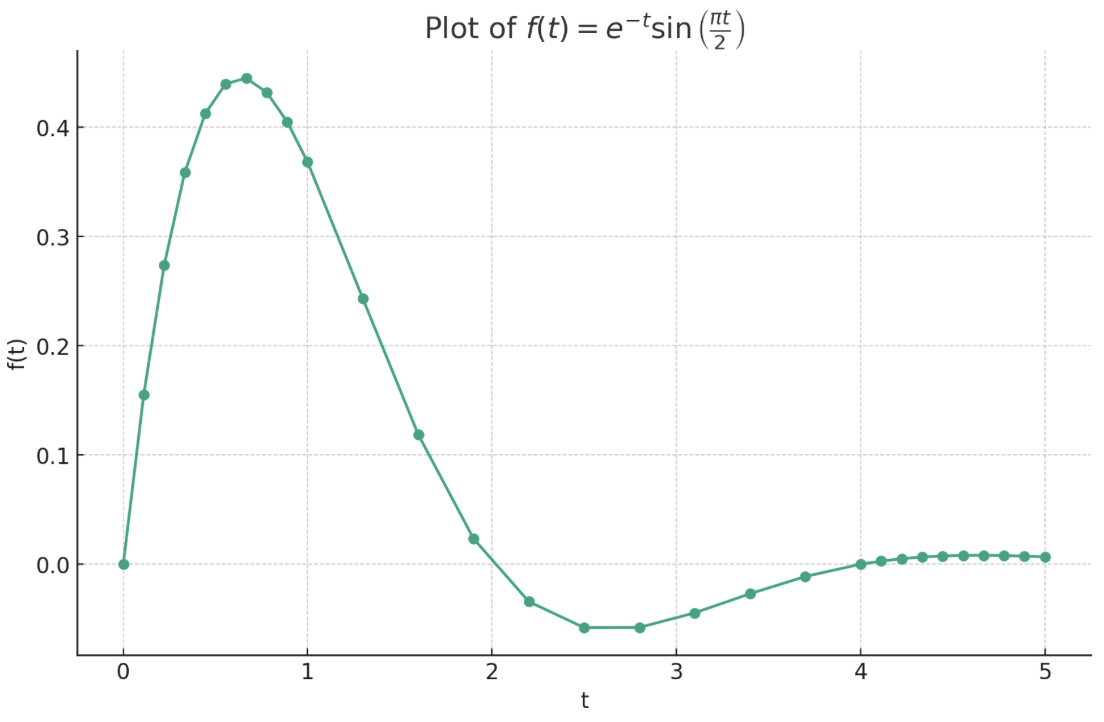
\includegraphics[width=0.65\linewidth]{lo.png}
\\
I've created Lagrange interpolations of the function $f(t)=e^{-t} \sin \left(\frac{\pi t}{2}\right)$ for different integer values of $n$ on each interval: $[0,1],(1,4)$, and $[4,5]$. (Not sorted, sorry. Latex was messing)
\\
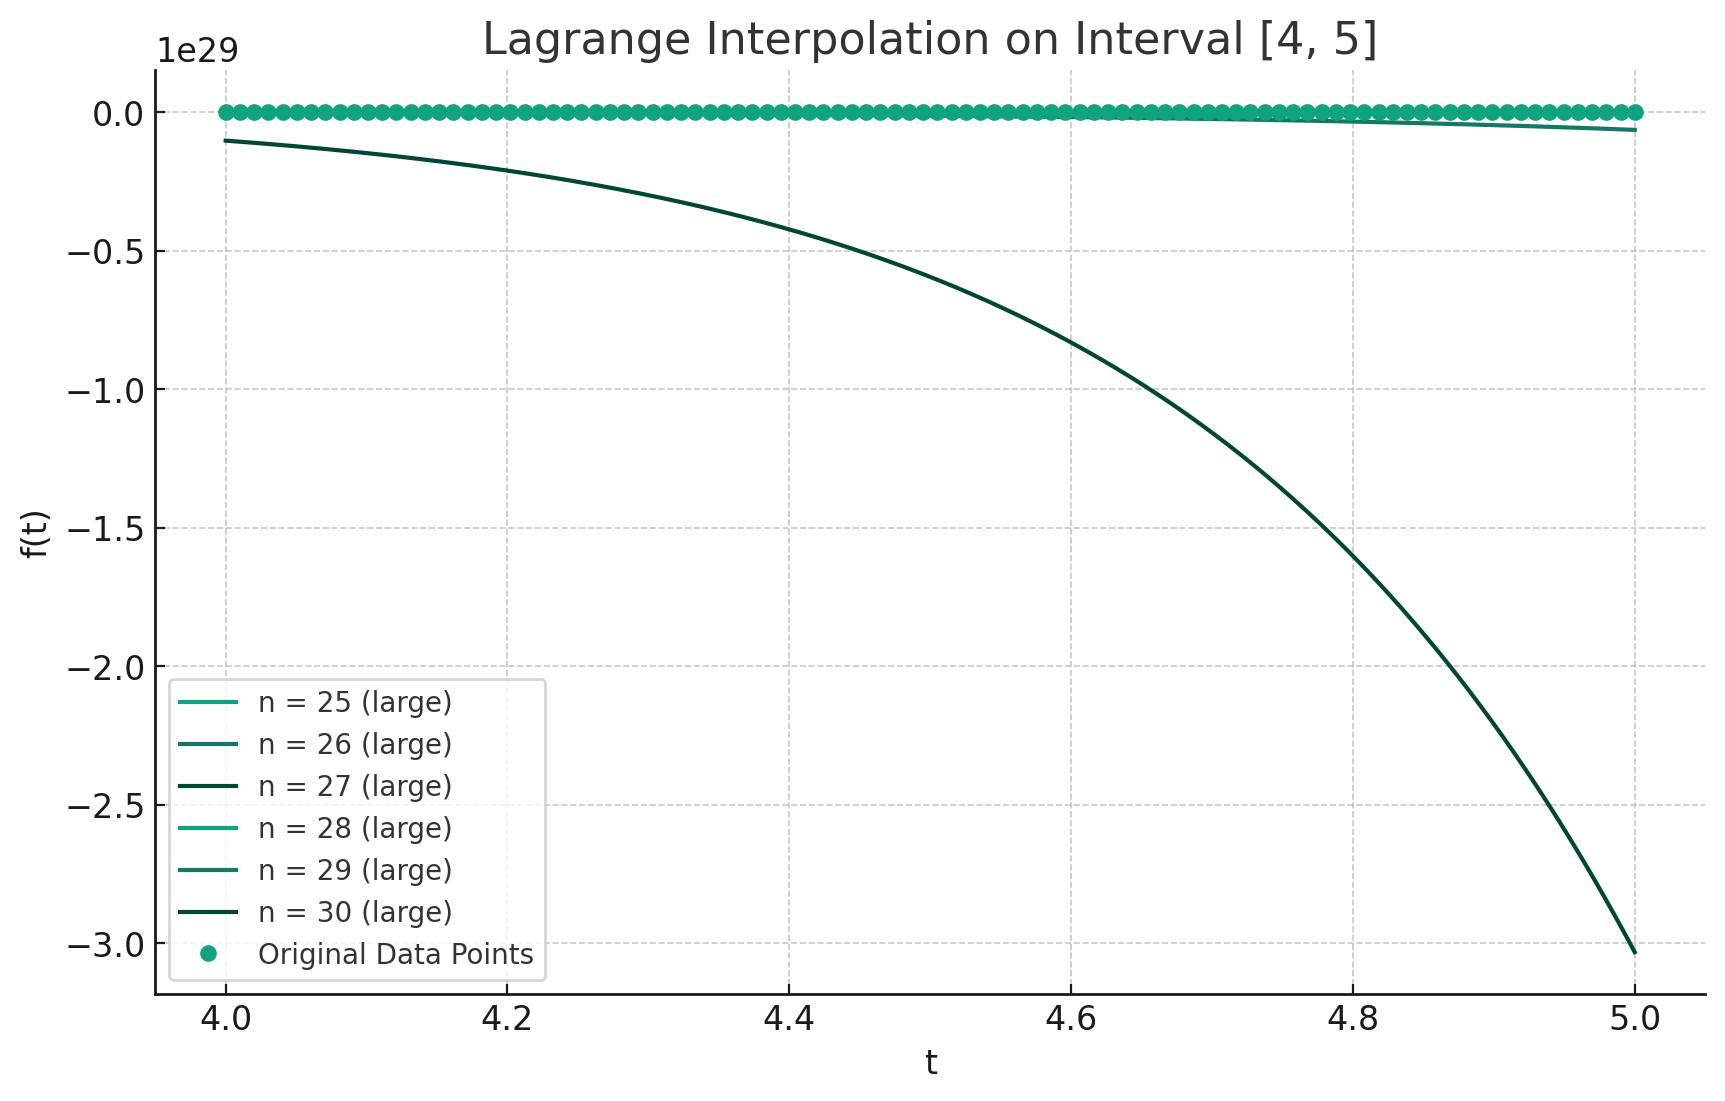
\includegraphics[width=0.40\linewidth]{019ad5c5-bbac-4b61-a609-ec57bd13db91.png}
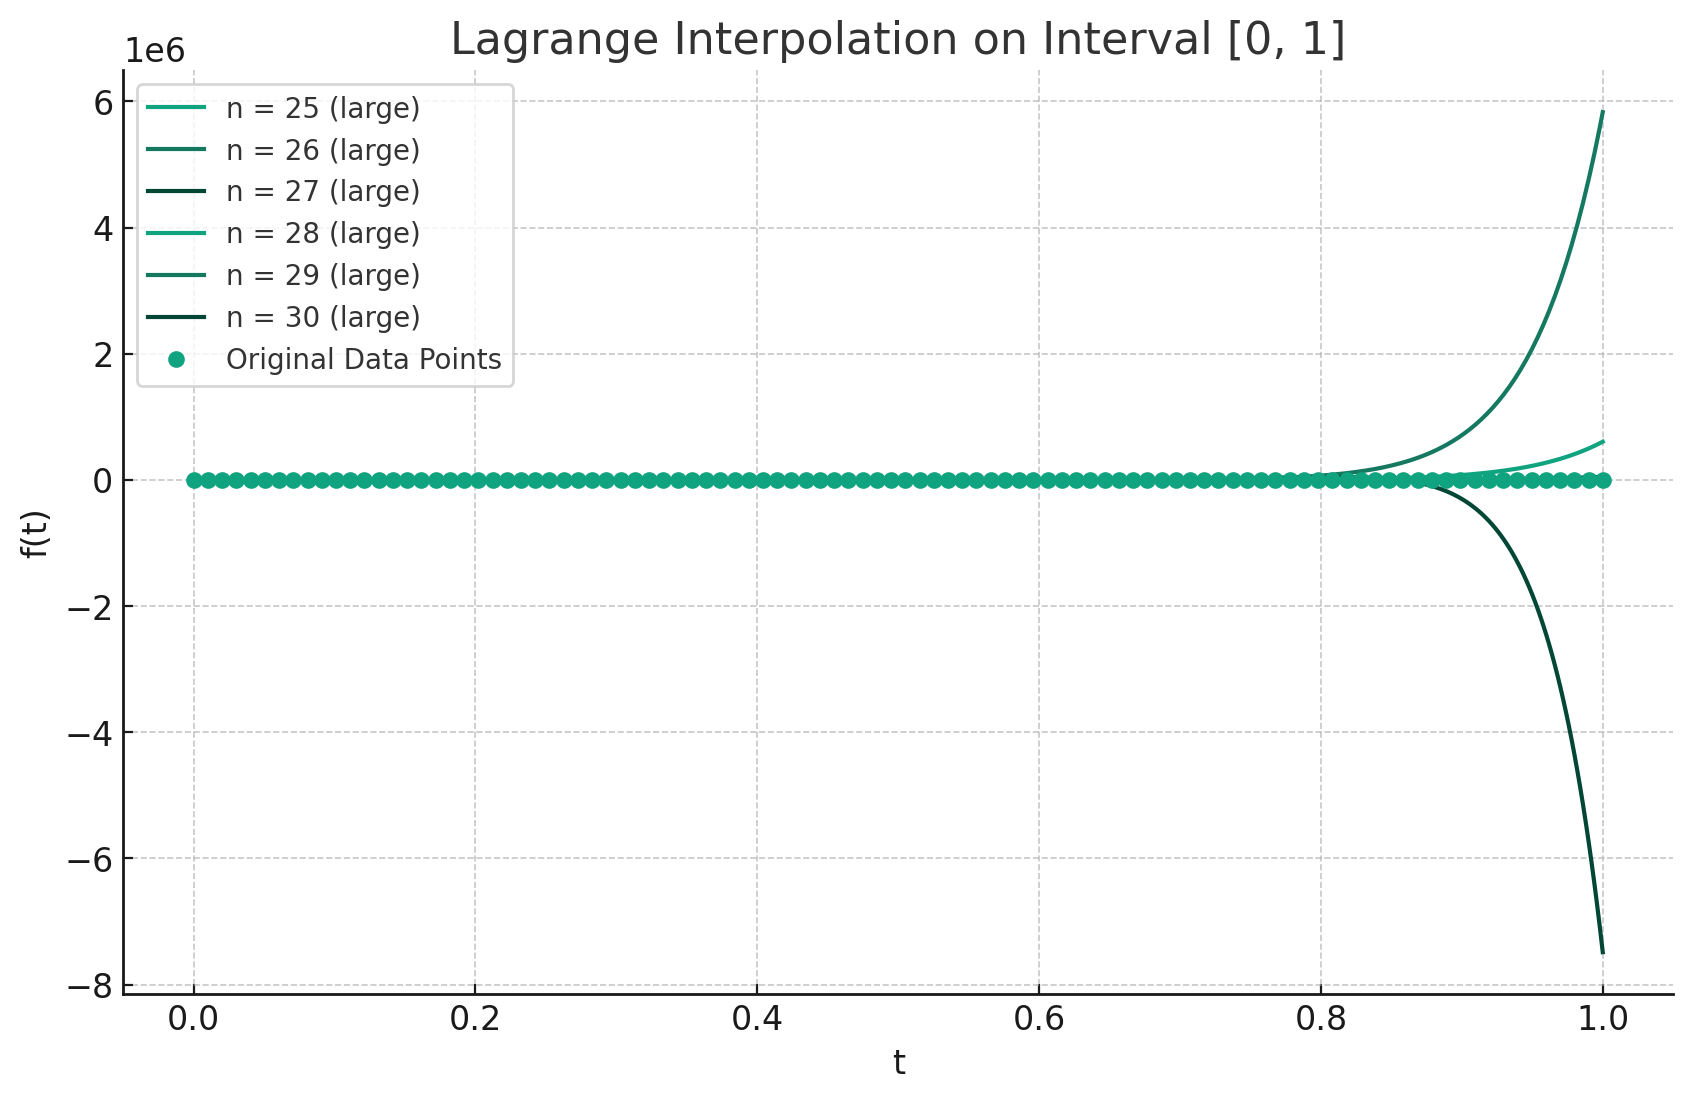
\includegraphics[width=0.40\linewidth]{27aa444b-d0d8-4259-be58-a1f20a6aefc7.png}
\\
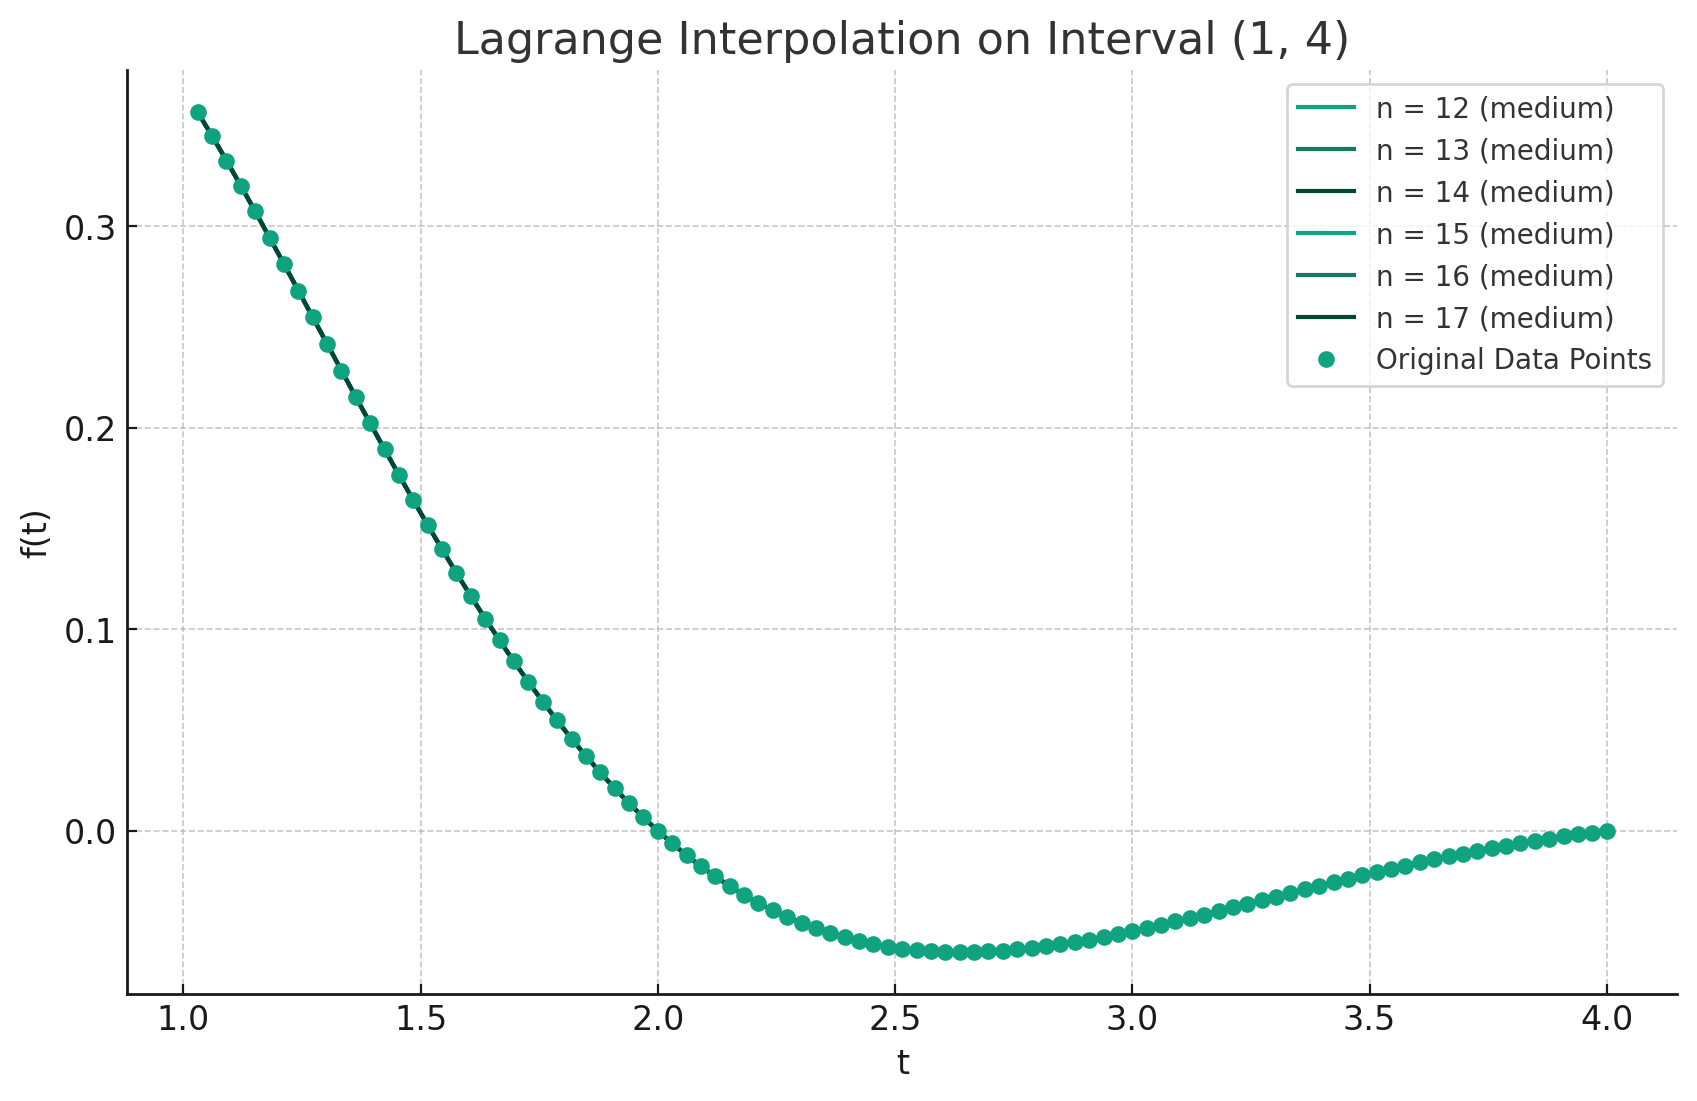
\includegraphics[width=0.40\linewidth]{39b2e0a0-8527-4e55-8e89-8cf0357719ce.png}
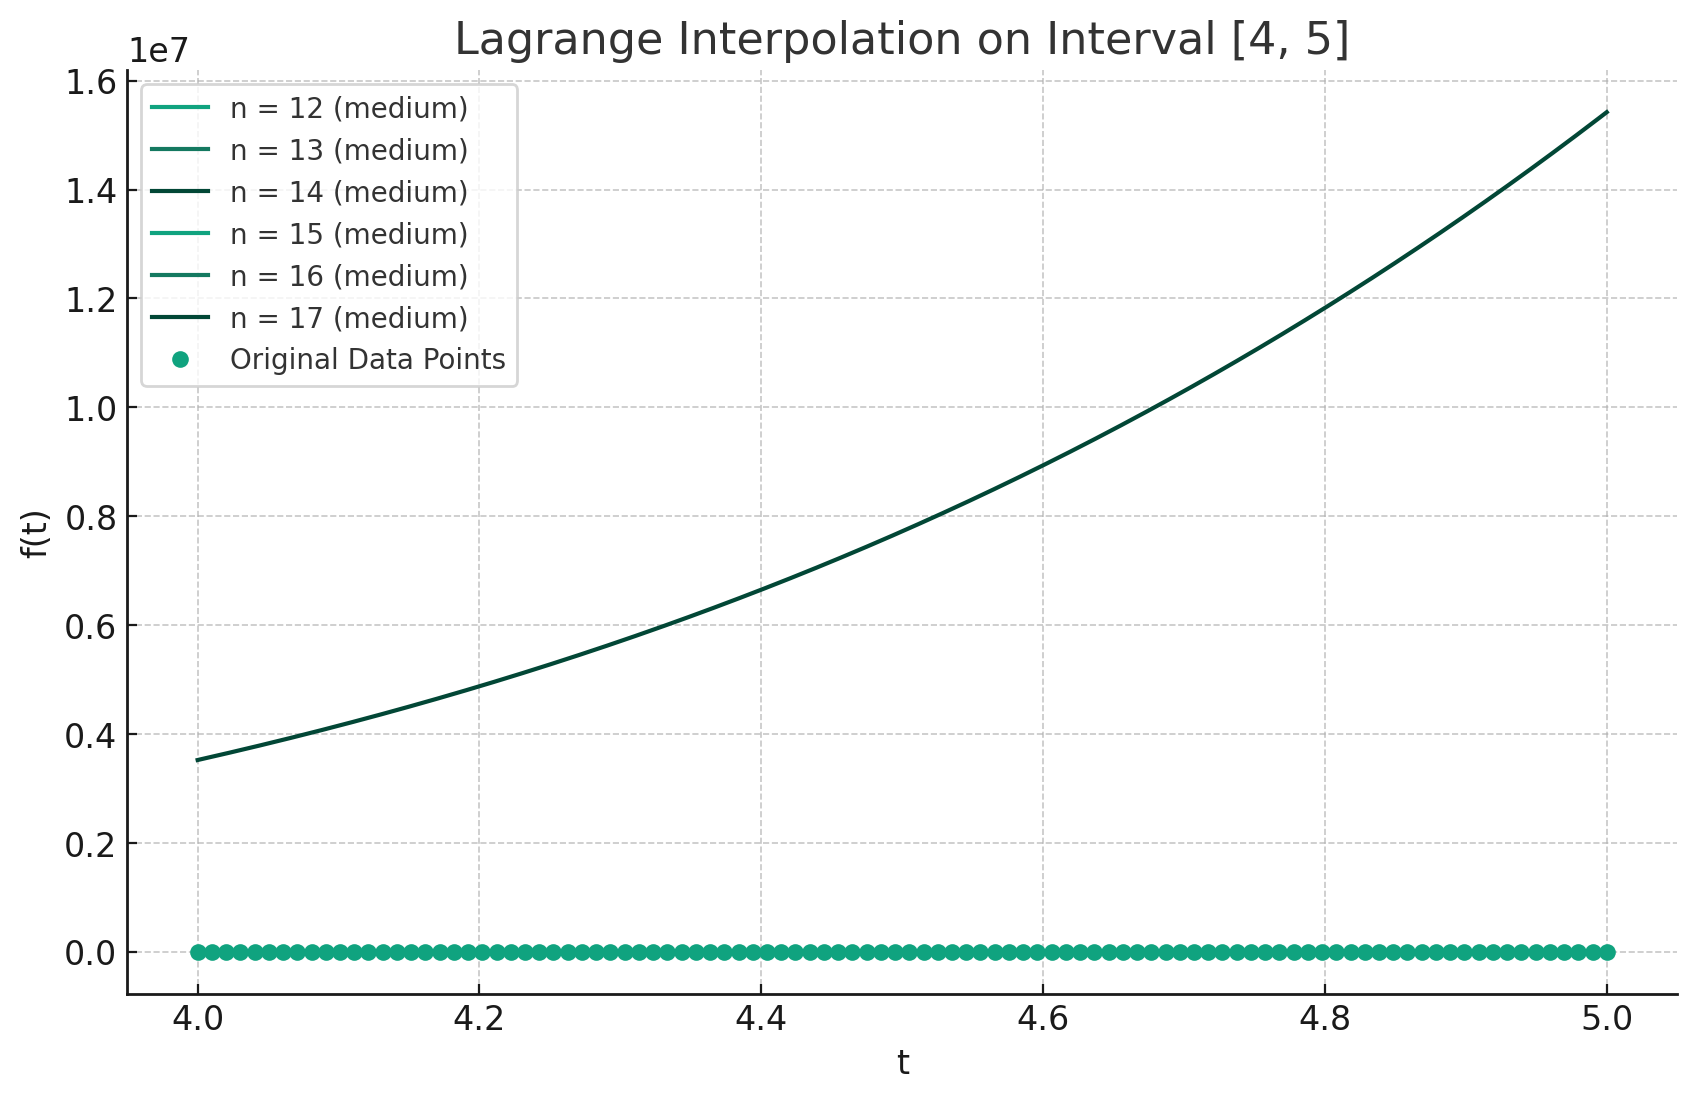
\includegraphics[width=0.40\linewidth]{80dc5fba-02be-4012-8f53-de8fbe24e1de.png}
\\
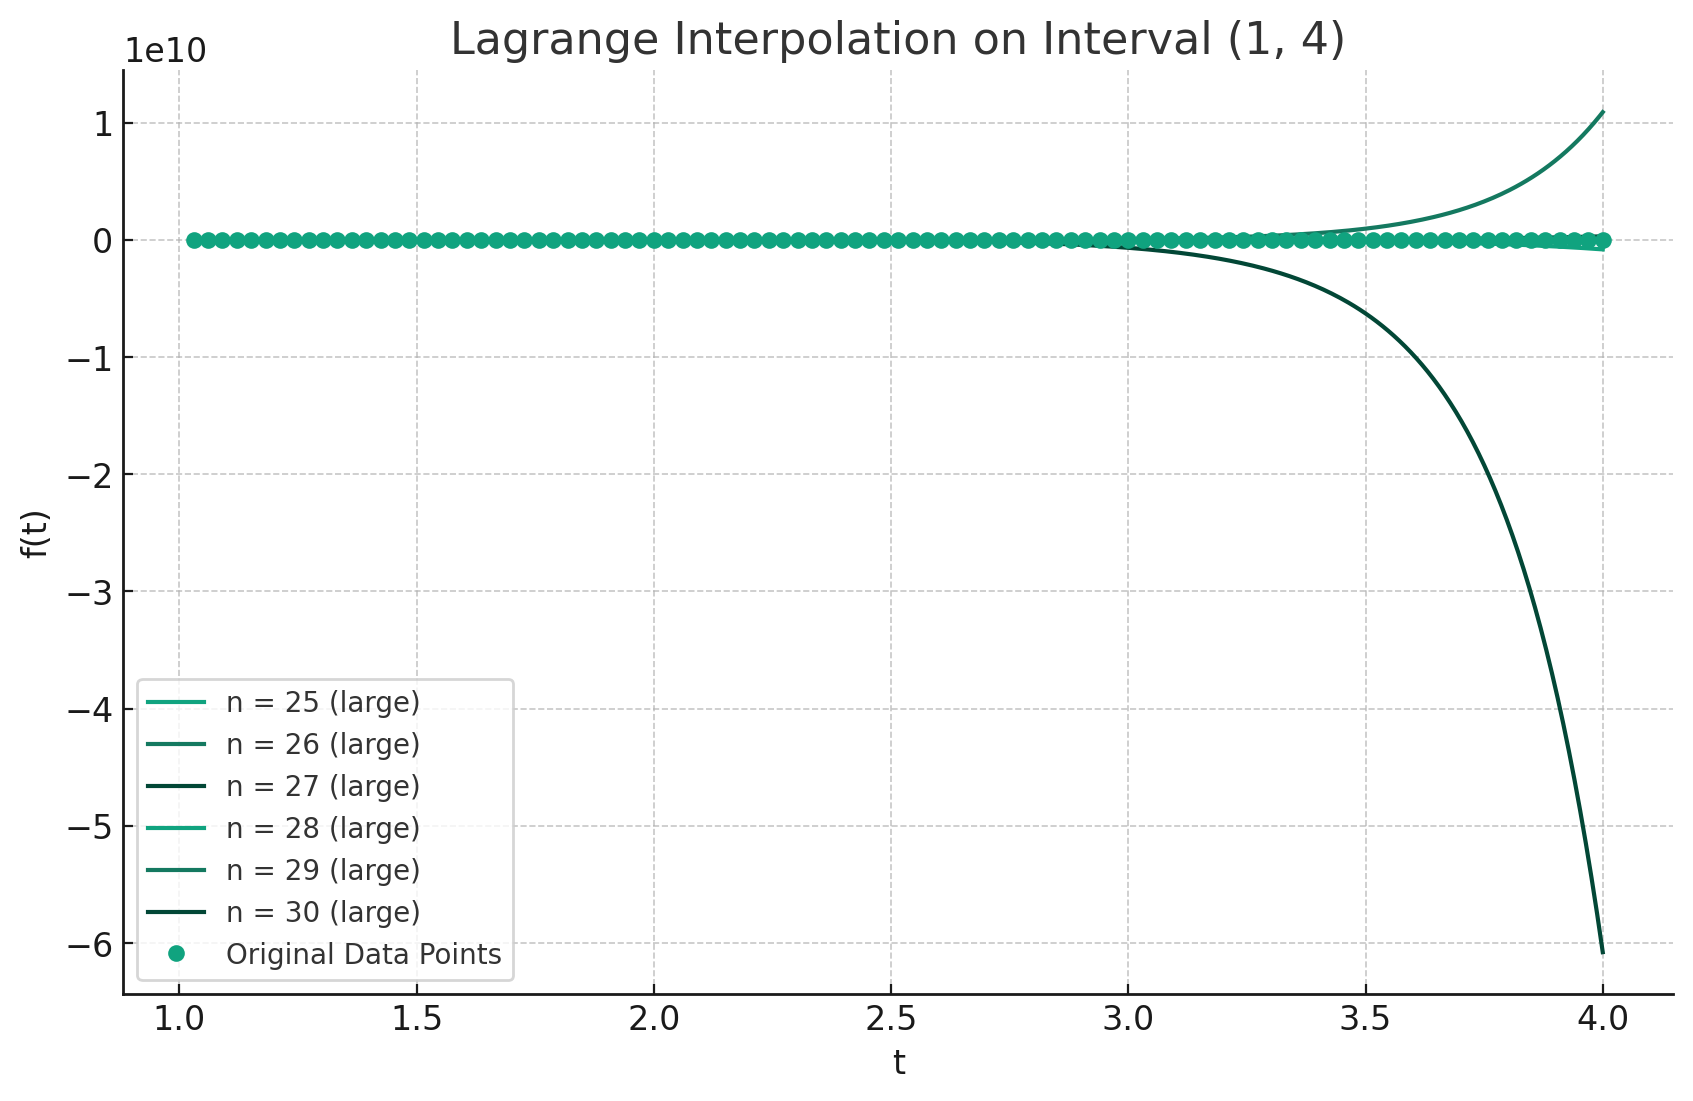
\includegraphics[width=0.40\linewidth]{404a68dd-4001-443a-bc02-5dd68d2ec4eb.png}
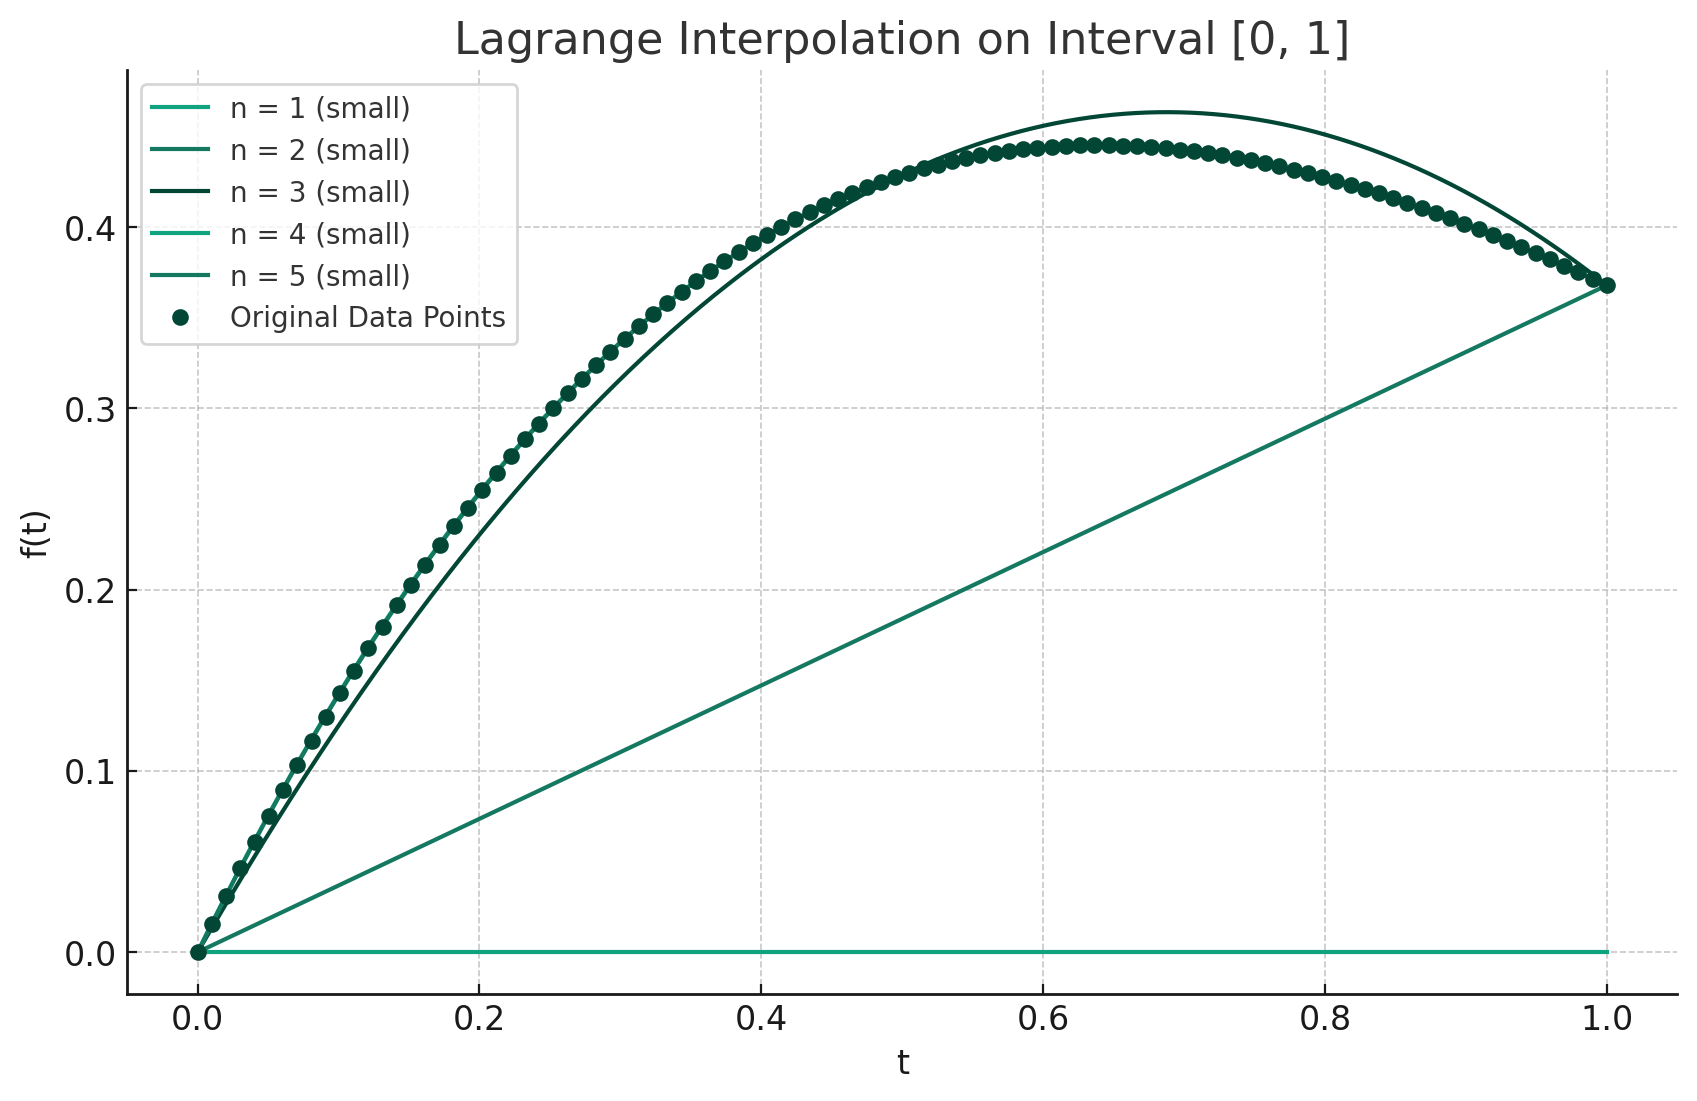
\includegraphics[width=0.40\linewidth]{66979bf9-479b-4f22-8c66-c47afcff914f.png}
\\
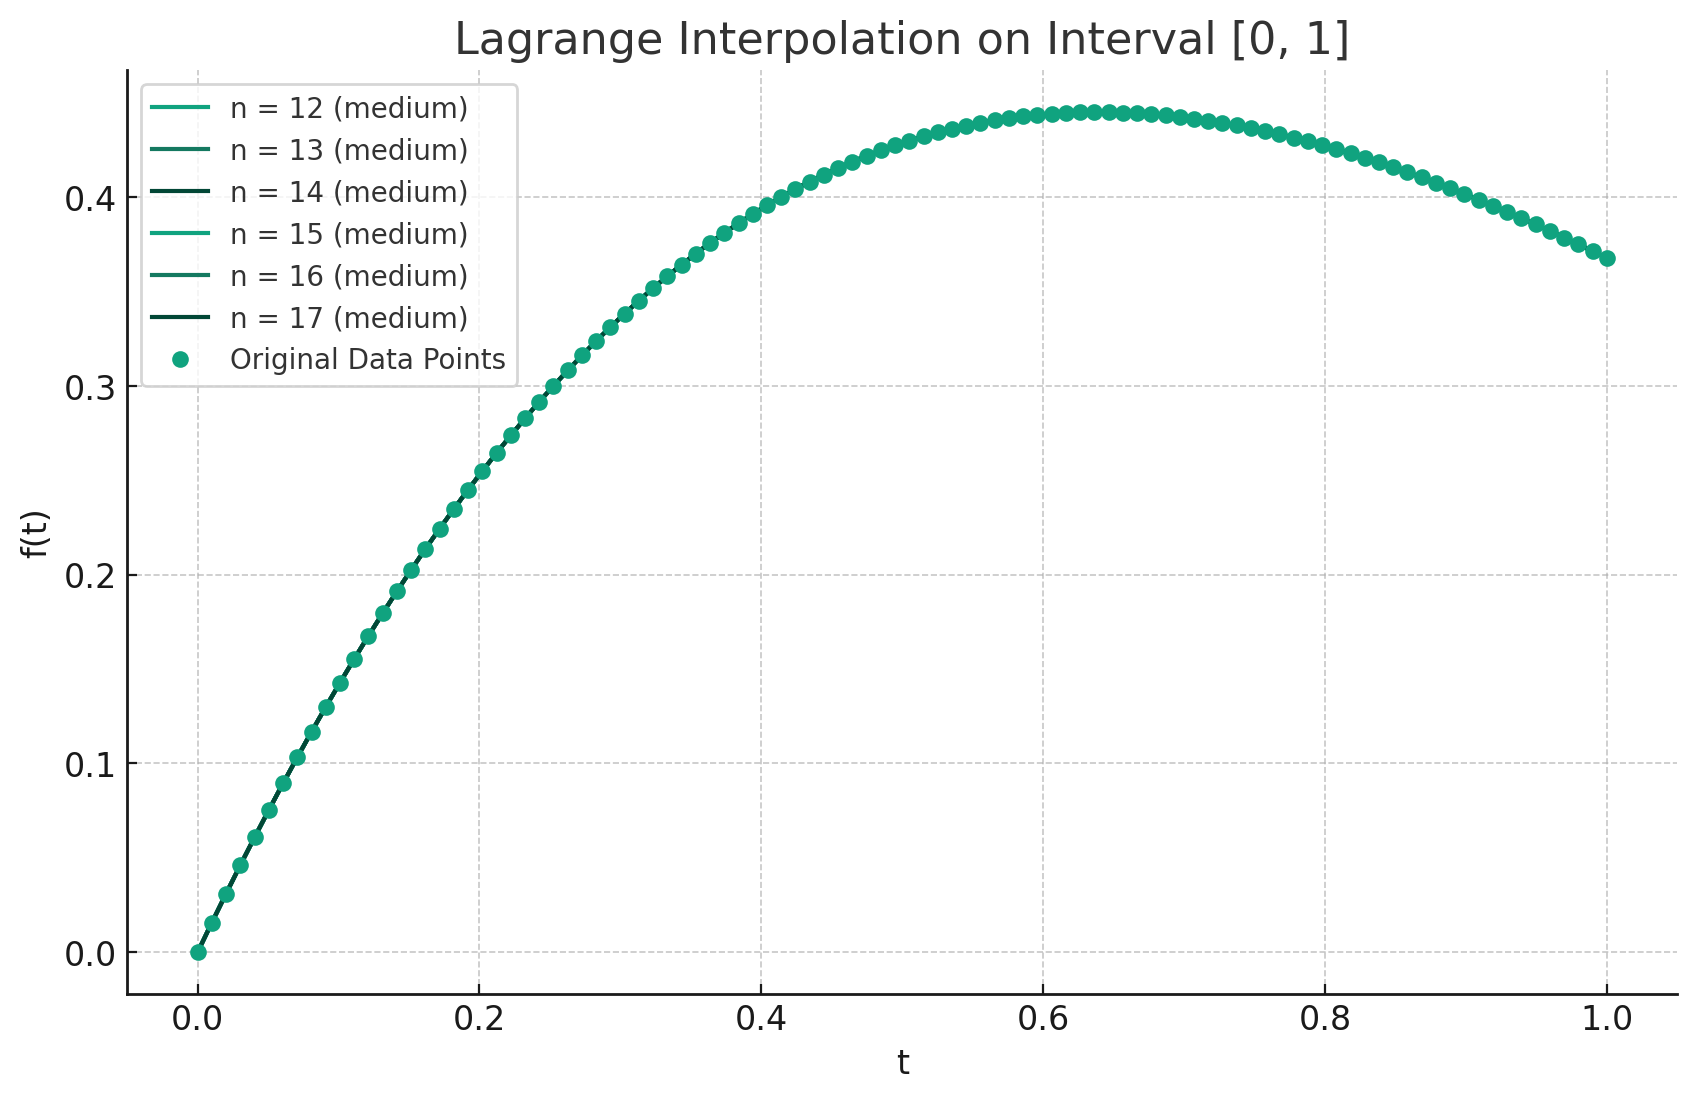
\includegraphics[width=0.40\linewidth]{a56c048e-0368-4d1f-8131-5d1bb6170e03.png}
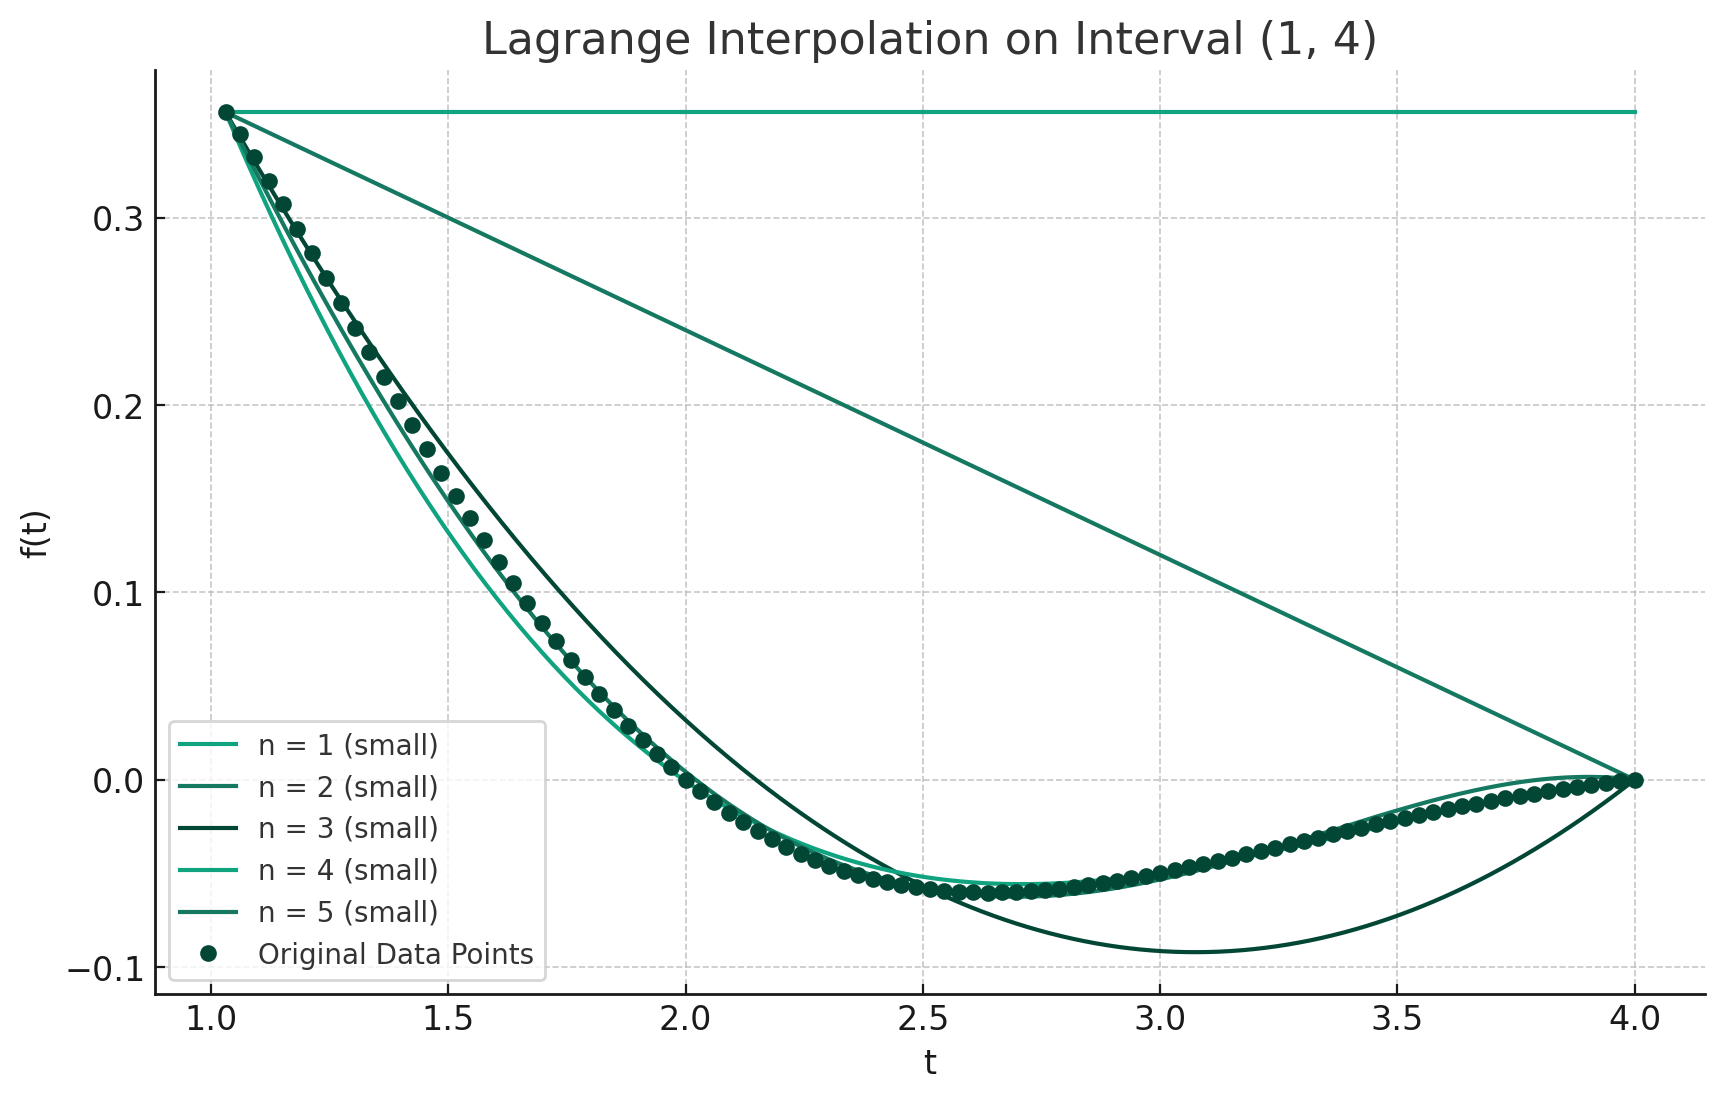
\includegraphics[width=0.40\linewidth]{bebe82e7-8293-433f-a54e-a9e0752c7139.png}
\\
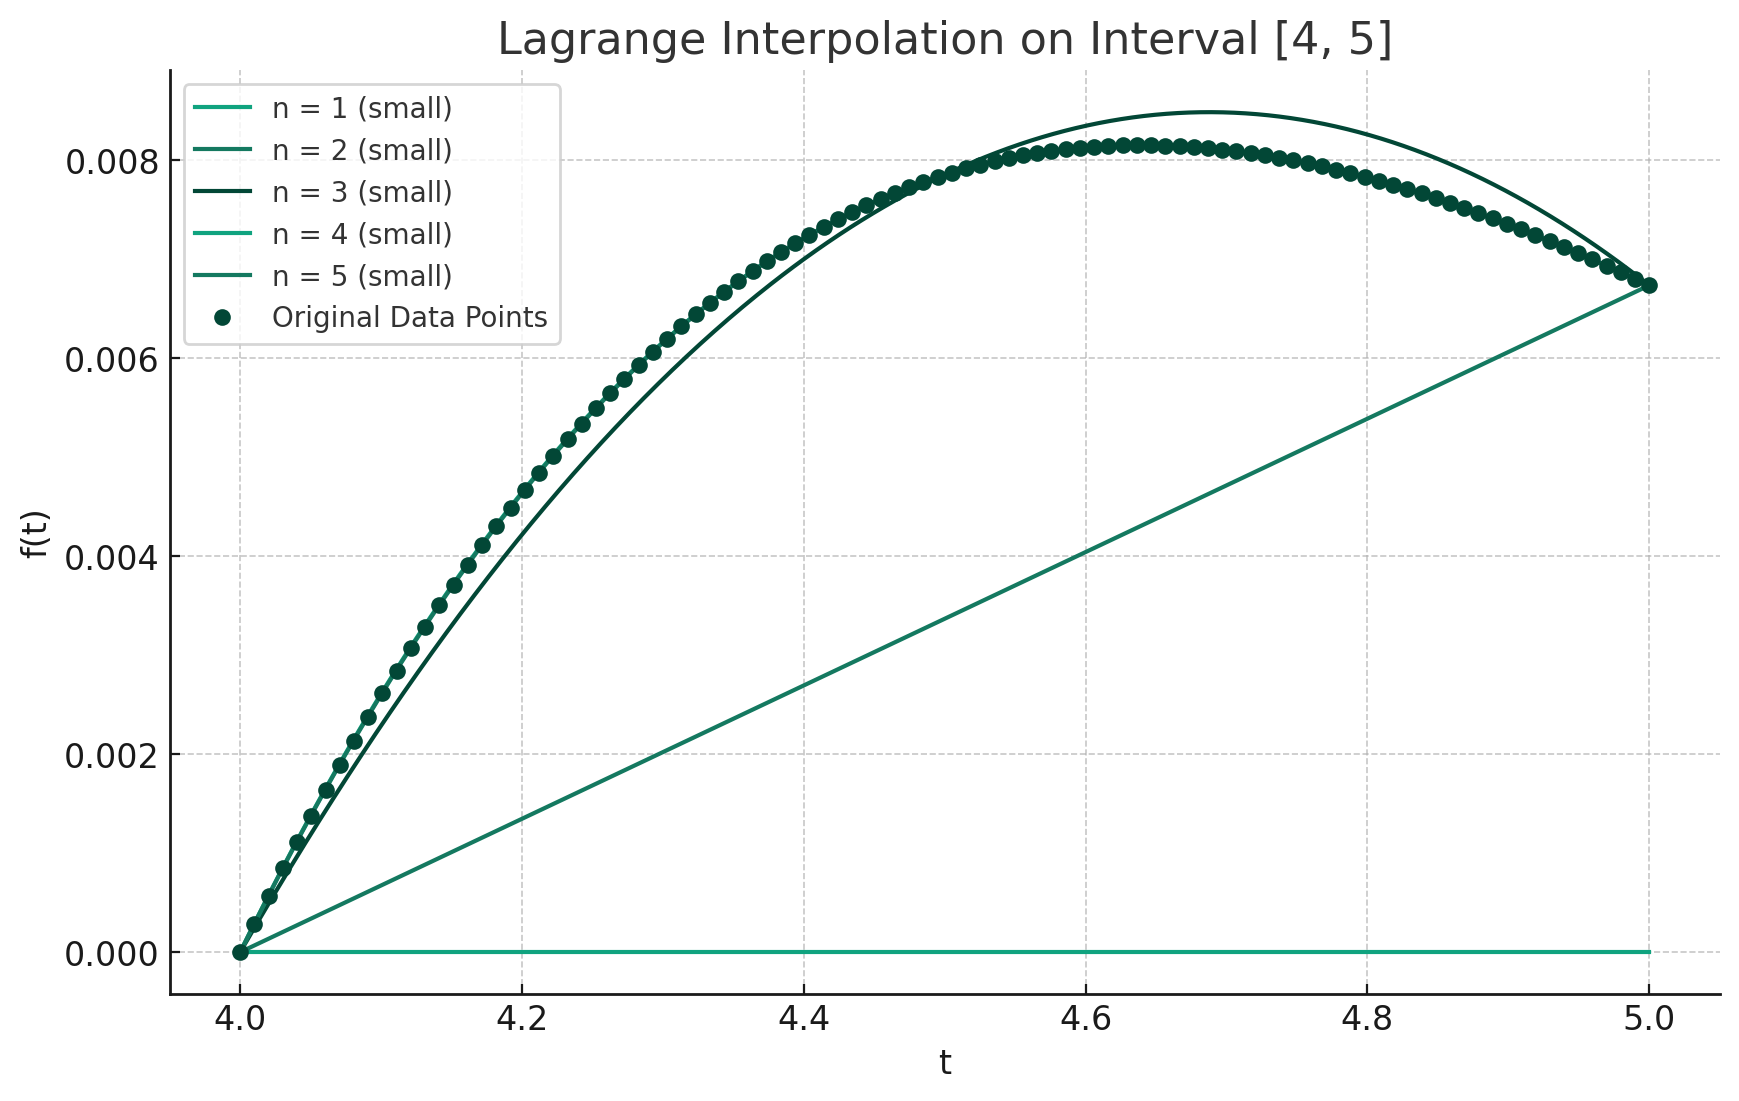
\includegraphics[width=0.40\linewidth]{fe83f5b2-0e16-4743-8783-9daeeda3d766.png}
\\
I've estimated the error $\left|f(t)-p_n(t)\right|$ for each natural number $n$ from 1 to 30 , following the $x$-value spacing rule described earlier. The plot shows the maximum absolute difference (estimated error) between the actual function $f(t)$ and its Lagrange interpolation $p_n(t)$ for $t$ in the interval $[0,3]$:
\\
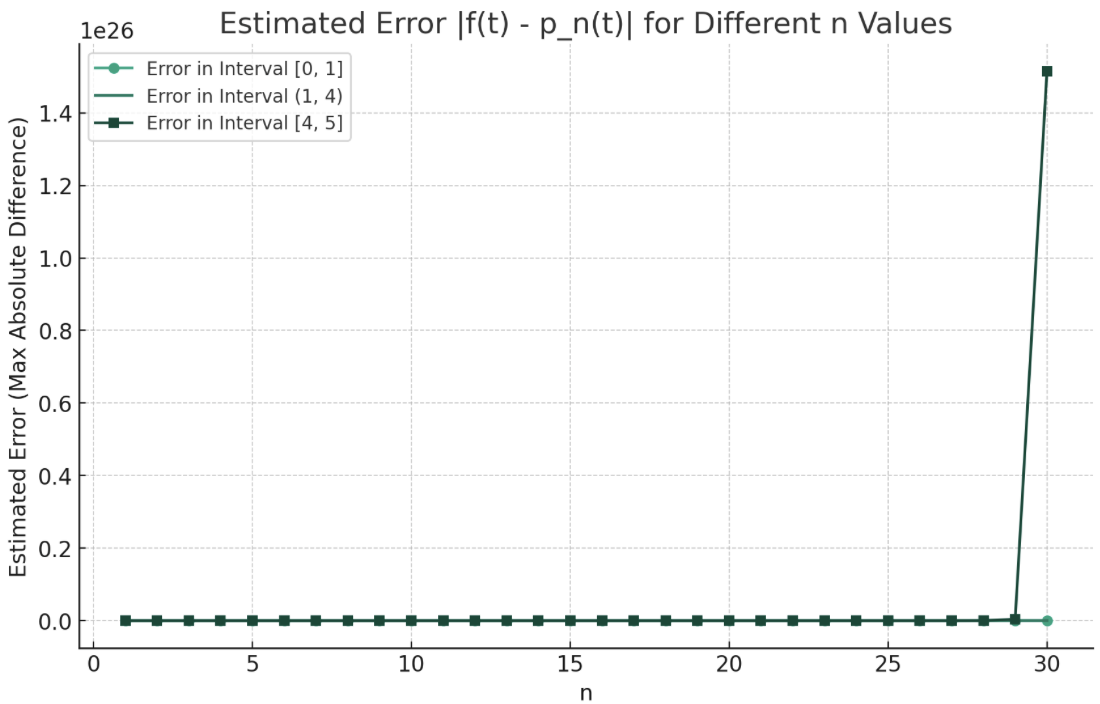
\includegraphics[width=0.60\linewidth]{123.png}

\section{problem 4}

\end{document}




\end{document}
\endinput
%%
%% End of file `sample-authordraft.tex'.
